\paragraph{Stacked function calls} Functions that calculate and return something can also call other functions that return something. Tracing might look like below. Using red digits, we indicate the order in which the trace is done.

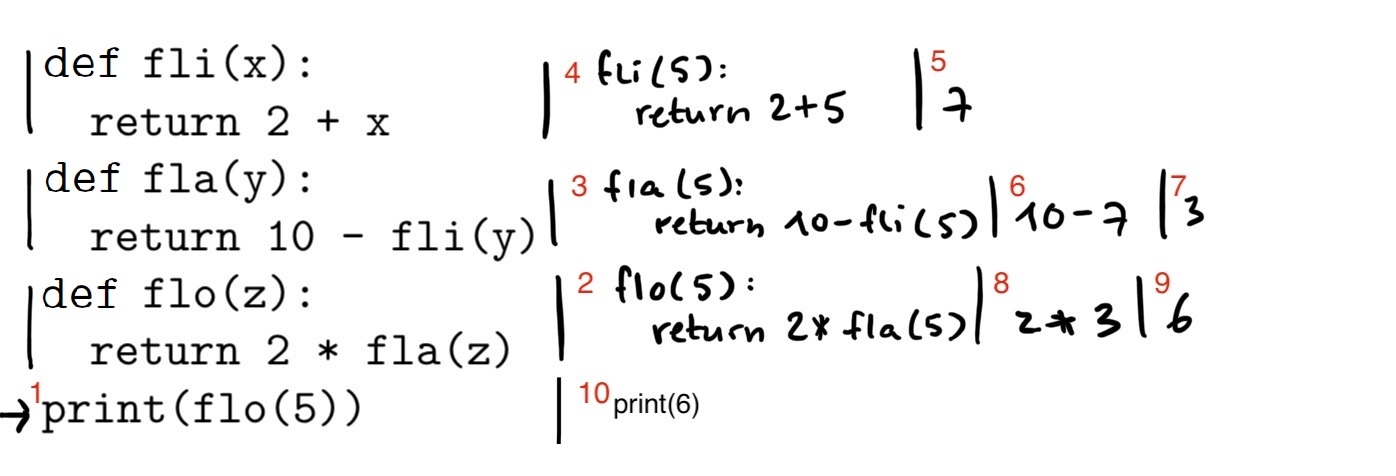
\includegraphics[width=.9\textwidth]{7-trace-multi-returns.jpeg}

Starting from the \texttt{print}, we see that the function \texttt{flo} is called with the value \texttt{5}. The function \texttt{flo} returns two times the result of the function \texttt{fla}, which is called with the variable \texttt{z} that has the value \texttt{5}. We can see that the function \texttt{fla} returns ten minus the result of the function \texttt{fli}, with the variable \texttt{y}, which has the value \texttt{5}. The function \texttt{fli} returns two plus the variable \texttt{x}, which has the value \texttt{5}. The outcome of \texttt{2 + 5 = 7}, so we can use back substitution to replace \texttt{fli(5)} with \texttt{7}. Now, we can calculate \texttt{10 - 7 = 3}, which means we can then replace \texttt{fla(7)} with \texttt{3}. Finally, we can calculate \texttt{2 * 3 = 6}, which is then substituted into the print.
